\section{Indgangsvinkel}
\label{DatabehandlingRIndgangsvinkel}




%
\begin{figure}[H]
\centering
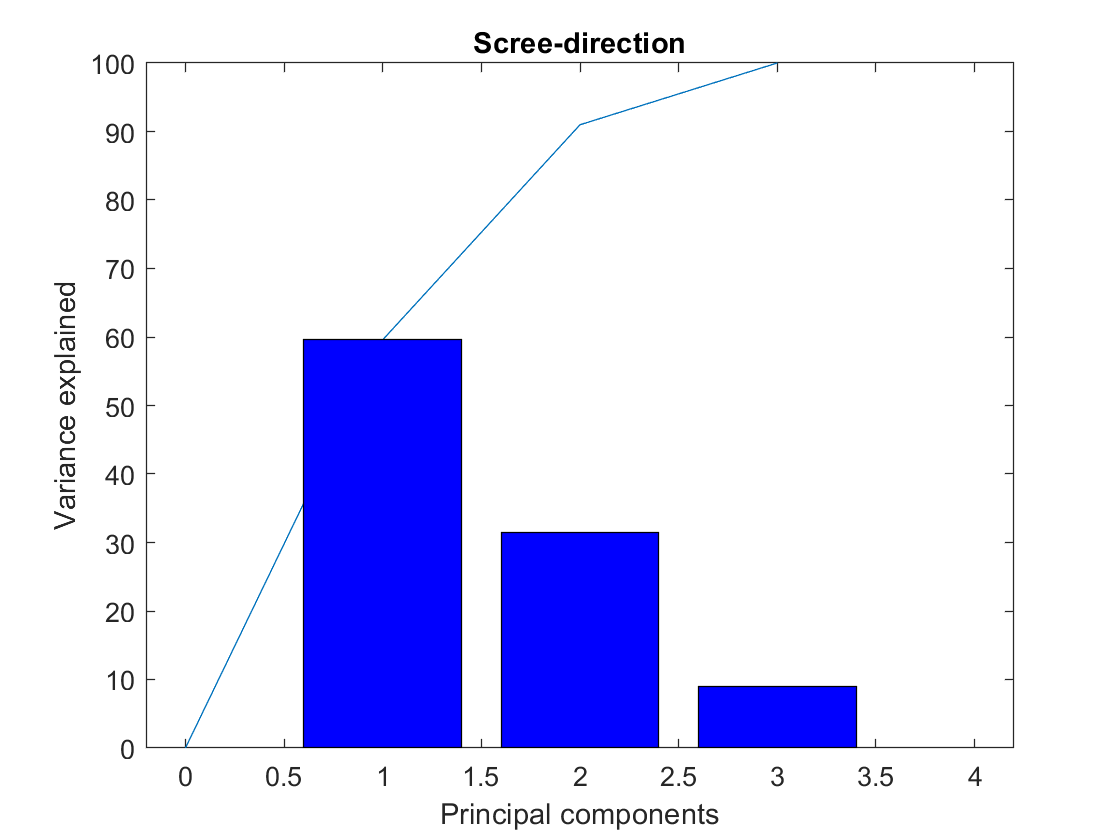
\includegraphics[width=\textwidth]{Figure/DatabehandlingSkalaer/PCAfigures/Direction-Scree.png}
\caption{\textit{Scree}-plot, hvorpå sammenhængen mellem antallet af \textit{Principal Components} og \textit{Variance Explained [\%]} fremgår.}
\label{fig:Direction-Scree}
\end{figure}
\noindent
%


%
\begin{figure}[H]
\centering
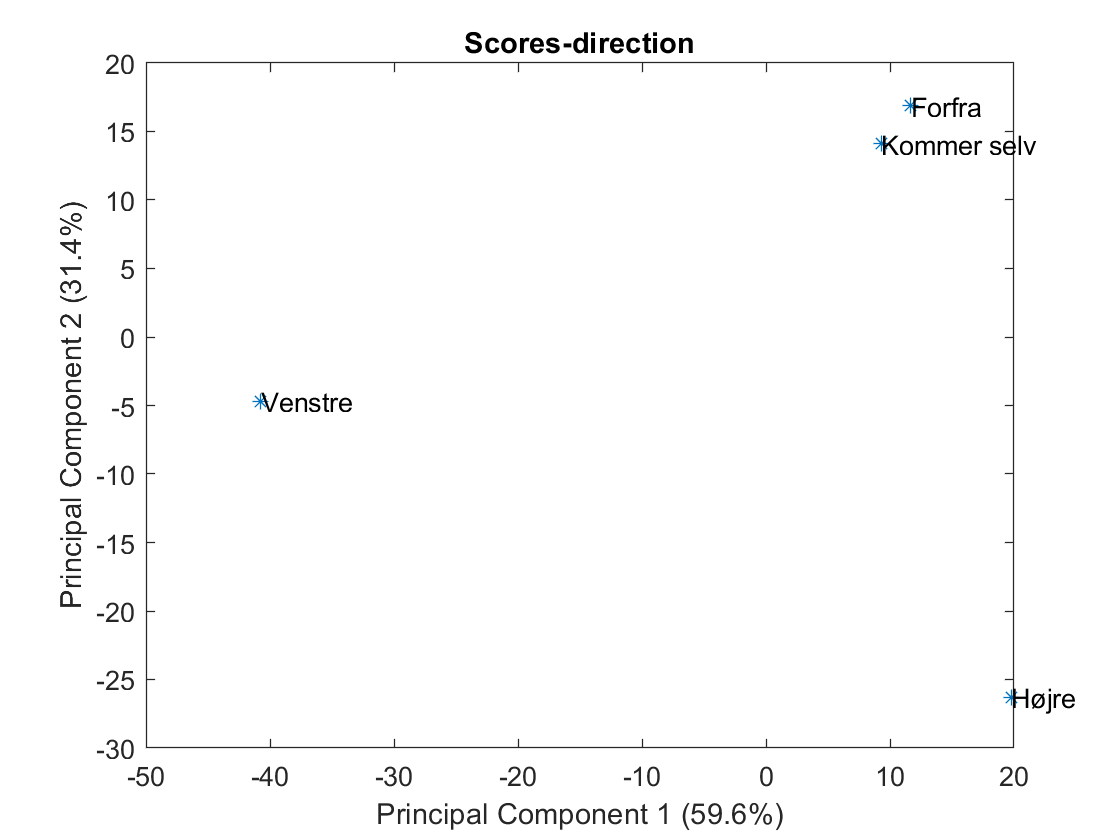
\includegraphics[width=\textwidth]{Figure/DatabehandlingSkalaer/PCAfigures/Direction-Scores}
\caption{\textit{Score}-plot for PC1 og PC2 i forhold til de tre afstande robotten holder til testpersonerne.}
\label{fig:Direction-Score}
\end{figure}
\noindent
%


SQ10 størst indflydelse på PC1
SQ1, SQ20 og SQ22 størst indflydelse på PC2

SQ18 + SQ20 korrelation
SQ8 + SQ10 korrelation
SQ9 + SQ14 korrelation
SQ4 + SQ13 korrelation 
SQ1 + SQ16 korrelation
SQ5 + SQ7 + SQ17 korrelation

SQ1 + SQ12 negativ korrelation
SQ21 + SQ22 negativ korrelation
SQ9 og SQ14 + SQ8 +SQ10 negativ korrelation
SQ6 + SQ23 negativ korrelation



%
\begin{figure}[H]
\centering
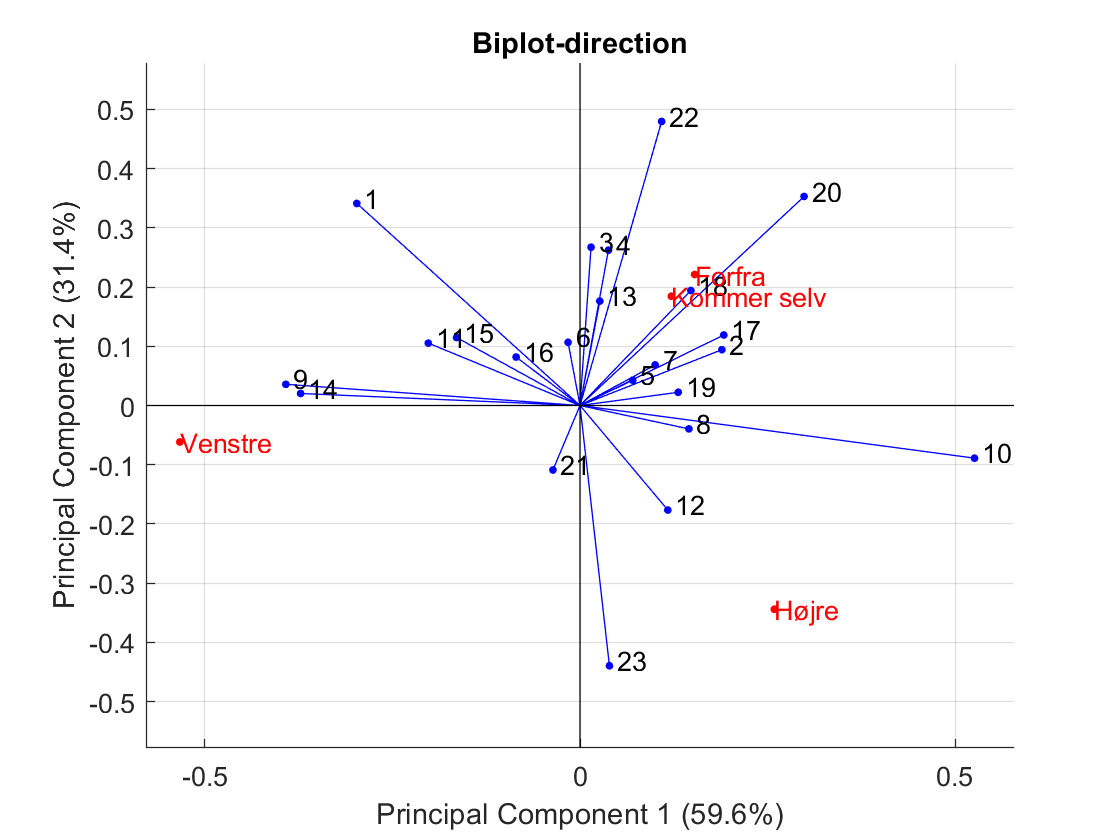
\includegraphics[width=\textwidth]{Figure/DatabehandlingSkalaer/PCAfigures/Direction-Biplot.png}
\caption{\textit{Bi}-plot med både \textit{loadings} (angivet med blå) og \textit{scores} (angivet med rød) fremgår i forhold til robottens indgangsvinkel.}
\label{fig:Direction-Biplot}
\end{figure}
\noindent
%

TABEL MED LOADINGS
%
\begin{table}[H]
\centering
\begin{tabular}{c|c|c|c}
    & PC1 (59.6\%)    & PC2 (31.4\%)    & PC3 (9\%)       \\ \hline
SQ1  & -0.2974         & 0.3412          & -0.2362         \\ \hline
SQ2  & 0.1890          & 0.0942          & -0.1122         \\ \hline
SQ3  & 0.0147          & 0.2673          & -0.0454         \\ \hline
SQ4  & 0.0379          & 0.2624          & 0.2993          \\ \hline
SQ5  & 0.0702          & 0.0427          & 0.0823          \\ \hline
SQ6  & -0.0159         & 0.1067          & 0.0165          \\ \hline
SQ7  & 0.1001          & 0.0686          & -0.0203         \\ \hline
SQ8  & 0.1451          & -0.0395         & 0.0291          \\ \hline
SQ9  & -0.3921         & 0.0358          & 0.0498          \\ \hline
SQ10 & \textbf{0.5258} & -0.0889         & -0.1395         \\ \hline
SQ11 & -0.2022         & 0.1053          & 0.3059          \\ \hline
SQ12 & 0.1170          & -0.1765         & 0.2387          \\ \hline
SQ13 & 0.0264          & 0.1764          & -0.4342         \\ \hline
SQ14 & -0.3724         & 0.0203          & 0.1812          \\ \hline
SQ15 & -0.1644         & 0.1147          & -0.2624         \\ \hline
SQ16 & -0.0851         & 0.0818          & 0.0851          \\ \hline
SQ17 & 0.1916          & 0.1191          & -0.1870         \\ \hline
SQ18 & 0.1478          & 0.1942          & 0.0192          \\ \hline
SQ19 & 0.1309          & 0.0223          & 0.2178          \\ \hline
SQ20 & 0.2987          & 0.3530          & \textbf{0.4448} \\ \hline
SQ21 & -0.0361         & -0.1089         & 0.2298          \\ \hline
SQ22 & 0.1088          & \textbf{0.4797} & -0.1187         \\ \hline
SQ23 & 0.0392          & -0.4395         & -0.1192        
\end{tabular}
\caption{Indgangsvinkel}
\label{tab:LoadingsIndgangsvinkel}
\end{table}
\noindent
%



TIL 3D plot 

SQ18 SQ20 er ikke positiv korrelation 
SQ13 + SQ4 er ikke positiv korrelation 
SQ1 + SQ16 er ikke positiv korrelation 
SQ7 + SQ17 er ikke positiv korrelation 
SQ5 + SQ17 er ikke positiv korrelation 

SQ2 + SQ7 korrelation


SQ21 + SQ22 er ikke negativt korrelation 

SQ13 + SQ21 er negativt korrelation